\documentclass[german,version-2022-01]{uzl-thesis}


% Copy this file as a template for your thesis. You will have to take
% action at all places marked by
%
% !!!!!!!!!!!!!!!!!!!!!!!!!!!!!!!!!!
% !!! Your action is needed here !!!
% !!!!!!!!!!!!!!!!!!!!!!!!!!!!!!!!!!
%
% The first place your action is needed is the first line of this
% document:
%
%
% Language of the thesis:
%
% You must use either 'german' or 'english' above, depending on the
% language used in the main text. This will automatically setup a lot
% of things in the background.
%
%
% Version of the class:
%
% You must specify which version of the thesis class is to be
% used. This is important in case the class style changes in later
% years, but we still want an older thesis to look the same, even when
% things are changed in the class.
%
% Do not change or remove the version-xxxx key.
%
%
% Text encoding:
%
% Your thesis *must* be encoded in utf8 (unicode), which is the
% default in most editors these days. Do *not* change this to latin8.



%%%
%
% Main setup:
%
%%%
%
% You must use the \UzLThesisSetup command to specify numerous things
% about your thesis. This includes the entries on the title page, the 
% abstracts, and the bibliography style. You do so by specifying
% so-called "values" for so-called "keys". For instance, 
% for the key "Autor" you must provide your name as the value. You do
% so by writing 'Autor = {Max Mustermann}', that is, the value is put
% into curly braces. You can use the \UzLThesisSetup command
% repeatedly and the order in which you provide the keys is not
% important. 
%
% Everything shown on the title page must be in German -- even
% if the thesis is written in English! Just insert German text for
% German keys and English text for English keys (like 'Abstract' needs
% English text, while 'Zusammenfassung' needs German text).

\UzLThesisSetup{
  %
  % !!!!!!!!!!!!!!!!!!!!!!!!!!!!!!!!!!
  % !!! Your action is needed here !!!
  % !!!!!!!!!!!!!!!!!!!!!!!!!!!!!!!!!!
  %
  % First, specify the institut or clinic at which the thesis was
  % written. You get the logo file from them (make sure it has the
  % correct size, namely the same as the example). If they do not have
  % a logo, the university's default logo is used.
  %
  % The 'verfasst' gets two arguments. Change the first to {an der}
  % for clinics, as in 'Verfasst = {an der}{Medizinischen Klinik I}'
  %
  Logo-Dateiname        = {uzl-thesis-logo-uzl.pdf},
  Verfasst              = {am}{Institut f\"ur Neuro- und Bioinformatik},
  %
  % The titles:
  %
  Titel auf Deutsch     = {
    Analyse einer DNA-Datenbank auf Mutationsstabilit\"at basierend auf (bio-)chemisch relevanter Molek\"uleigenschaften
  }, 
  Titel auf Englisch    = {
    Analysis of a DNA Database for Mutation Stability Based on (Bio-)Chemically Relevant Molecular Properties 
  },
  %
  % Author and supervisor:
  % 
  % Note that the 'Betreuer' or 'Betreuerin' is the supervisor, that
  % is, the professor who officially supervises the thesis. If there
  % is also an assistent of the professor who helped (typically a
  % lot), use 'Mit Unterstützung von' to thank that person. If the
  % thesis was mainly written 'externally' at some company or another
  % institute, point this out using 'Weitere Unterstützung'. 
  % 
  % For your own name, do *not* add things like "BSc" or "BSc
  % cand.". For the supervisor, you should normally include
  % "Prof. Dr." or "PD Dr." (ask your supervisor, what is
  % appropriate), but nothing more (so no
  % "Univ.-Prof. Dr. Dr. h.c. mult." unless your supervisor insists).  
  %
  Autor                 = {Leonie Nie\ss{}},
  Betreuerin            = {PD Dr. Amir Madany Mamlouk},
  % 
  % Optional: Supporting persons and institutions. The text should be
  % in German, even for an English thesis.
  %
  Mit Unterstützung von = {BSc. Nina Eichler},
  % 
  %   Weitere Unterstützung = {
  %     Die Arbeit ist im Rahmen einer Tätigkeit bei der Firma Muster GmbH
  %     entstanden.
  %   },
  %
  %
  % Your Degree Programm (Studiengang)
  %
  % Specify 'Bachelorarbeit' or 'Masterarbeit' and the degree
  % programme. Make sure the name of programme is correct and not
  % some abbreviation or some incorrect variant. For instance:
  % 'Medizinische Ingenierwissenschaft', but not 'MIW';
  % 'Medizinische Informatik', but not 'Medizin-Informatik';
  % 'Informatik', but not 'Informatik (SSE)'.
  %
  % Use German names for German programmes and English names for
  % English ones, so 'Infection Biology', not 'Infektionsbiologie'. 
  % For programmes that have a German bachelor and an English master,
  % use the German name for a bachelor thesis and the English name for
  % the master thesis.
  %
  Bachelorarbeit,
  Studiengang           = {Medizinische Informatik},
  %
  % Date on which the thesis is turned in German, formatted the
  % traditional German way:
  %
  Datum                 = \today,
  %
  % The English abstract. You must always provide abstracts in German
  % and in English. 
  %
  Abstract              = {
  
  },
  Zusammenfassung       = {
  
  },
  %
  % Optional: 'Danksagungen' (German) or 'Acknowledgements'
  % (English). Both keys are optional and both have the same effect of
  % adding an acknowledgements text after the abstracts and before the
  % table of contents.
  %
  %Acknowledgements      = {
  %  This is the place where you can thank people and institutions, do not try to do this on the title page. The only exception is in case you wrote your thesis while working or staying at a company or abroad. Then you should use the \Latex{Weitere Unterstützung} key to provide a text (in German) that acknowledges the company or foreign institute. For instance, you could use texts like »Die Arbeit ist im Rahmen einer Tätigkeit bei der Firma Muster GmbH entstanden« or »Die Arbeit ist im Rahmen eines Forschungsaufenthalts beim Institut für Dieses und Jenes an der Universität Entenhausen entstanden«. Do not name and thank individual persons from the company or foreign institute on the title page, do that here. 
  %},
  % Bibliography style: Choose between
  % 
  % 'Alphabetische Bibliographie'
  % for all degree programmes in the natural sciences 
  % 
  % 'Numerische Bibliographie'
  % alternative for all other degree programmes
  % 
  % Either will load biblatex and setup the citation methods and the
  % bibliography styles correctly. You should not mess with them.
  % 
  % Alphabetische Bibliographie,
  % Alternatively:
  Numerische Bibliographie
}




%%%%%%%%%%%%%%%%%%%%
%
% Styling the thesis
%
%%%%%%%%%%%%%%%%%%%%
%
% Creating a visually pleasing layout and choosing fonts is not
% easy. Furthermore, different people have different preferences. Of
% course, for the University of Lübeck, the dean of studies could just
% force everyone to use one specific layout and font, but that seems a
% bit drastic and, also, it seems nice that thesis by different people
% have an individual style even though they all stick to the same
% overall structure.
%
% For these reasons, I (Till Tantau) have spend quite some time on
% designing a flexible layout and styling mechanism for theses.
%
% Basically, the overall structure of the thesis is fixed by the
% thesis class and so are many structural elements. For instance, you
% cannot change the order in which the abstract and table of contents
% are shown, you cannot move the bibliography elsewhere, indeed, the
% bibliography style is also fixed. Likewise, the text on the title
% page is fixed.
%
% Although many things are fixed, you *can* change several other
% things. For instance, you can change the font used for the main
% text, you can change which font is used for titles and headings or
% you can change whether titles and headlines are centered or flushed
% left.
%
% There are many LaTeX packages for changing such things. You are
% kindly asked *not to use them*. Rather, use (only) the options
% offered by the thesis class. All possible choices and combinations
% there have been tested by me and produce nice results; what happens
% with other packages no one knows and might no longer conform to what
% is expected by the university. As you will see, you still have a
% lot of options.
%
%
% Technical note: All styling is done via the command
%
% \UzLStyle{...}
%
% where ... is a key-value list just as for \UzLThesisSetup. The
% difference is just that everything having to do with styling as
% controlled by \UzLStyle, while the more “formal” setup keys are
% controlled by \UzLThesisSetup.
%
%%%
%
% Designs
%
%
% A \emph{design} is a whole set of font and layout options bundled
% together. They have been chosen in such a way that a visually
% pleasing “overall appearance” results.
%
%
% \UzLStyle{computer modern oldschool design}
%
% The look of this design mimics the “classical” way a paper or report
% created with \LaTeX\ looks like: The Computer Modern font is used,
% bold face fonts are used for headlines, only black and white are
% used as colors. This design reminds me of older scientific
% documents, especially from the computer science community where
% \LaTeX\ was used very early.
%
%
% \UzLStyle{computer modern basic design}
%
% A slightly less “oldschool” version of the previous design. It is
% still a classic design in the sense that it uses the Computer Modern
% font and that it still has this “good old \LaTeX” look, but some
% more modern aspects (like colors!) have been added.
%
% Note that this design uses Myriad for the title page (one of the
% “modern aspect”), which means that his font must be installed.
%
%
% \UzLStyle{computer modern scholary design}
%
% In my opinion, this is the ultimate “scholary design”: The thesis
% will look like it has been typeset by hand some 150 years ago and
% then printed by a university press. There is really nothing “modern”
% about it and the word in the name of the design is just part of the
% name of the “Computer Modern” font.
%
%
% \UzLStyle{pagella basic design}
%
% A, well, basic design that uses the Pagella font rather than the
% Computer Modern font. Especially the bold face version of this font
% looks nicer than the Computer Modern counterpart. Also, Pagella,
% while still having a “bookish” look, still feels a bit fresher than
% Computer Modern. 
%
%
% \UzLStyle{pagella centered design}
%
% A variant of the basic Pagella design that centers all
% headlines. A nice alternative to the basic version.
%
%
% \UzLStyle{pagella contrast design}
%
% This design tries to create some visual friction by contrasting the
% sans serif headline font (in bold!) with the main text. I find it a
% visually very interesting combination.
%
%
% \UzLStyle{alegrya basic design}
%
% The third variant of the basic design, this time using the Alegrya
% font. 
%
%
% \UzLStyle{alegrya scholary design}
%
% The Alegrya version of the previous “scholary” design. Unlike the
% Computer Modern version, this design does not look old, but more
% fresh -- while still creating the impression that the text must be
% about a very scientific subject. 
%
%
% \UzLStyle{alegrya stylish design}
%
% The design is quite similar to the scholary version for the Alegrya
% font, but with even more modern additions. “Stylish” is the word
% that comes to my mind.
%
%
\UzLStyle{alegrya modern design}
%
% A design that uses the sans serif version of the Alegrya font for
% the headlines. This is a nice modern overall design.
%
%%%




%%%%%%%%
%
% Now, include the package you need here using \usepackage. 
%
% However, many standard packages are already loaded by the class:
%
% amsmath, amssymb, amsthm, babel, biblatex, csquotes, etoolbox,
% filecontents, fontspec, geometry, hyperref, tikz (with libraries
% arrows.meta, positioning and shapes), varioref, url 
%
% Indeed, in many cases you will not need any extra packages.
%
%%%%%%%





\begin{document}

%
% The title page and table of contents will be inserted automatically
% here. 
%


\chapter{Einleitung}
% In a German thesis write: \chapter{Einleitung}


% !!!!!!!!!!!!!!!!!!!!!!!!!!!!!!!!!!
% !!! Your action is needed here !!!
% !!!!!!!!!!!!!!!!!!!!!!!!!!!!!!!!!!
%
% Replace with your own introduction:


\section{Beitr\"age dieser Arbeit}
% In a German thesis write: \section{Beiträge dieser Arbeit}

% !!!!!!!!!!!!!!!!!!!!!!!!!!!!!!!!!!
% !!! Your action is needed here !!!
% !!!!!!!!!!!!!!!!!!!!!!!!!!!!!!!!!!
%
% Replace with a detailed account of your contributions:


\section{Verwandte Arbeiten}
% In a German thesis write: \section{Verwandte Arbeiten}

% !!!!!!!!!!!!!!!!!!!!!!!!!!!!!!!!!!
% !!! Your action is needed here !!!
% !!!!!!!!!!!!!!!!!!!!!!!!!!!!!!!!!!
%
% Replace with a detailed account of what other people have already
% researched concerning your thesis's theme. Even when (indeed,
% especially when) there has been only little or even no research by
% other people, you should explain in detail that this is the case and
% why it is the case. 


\section{Aufbau dieser Arbeit}
% In a German thesis write: \section{Aufbau dieser Arbeit}


% !!!!!!!!!!!!!!!!!!!!!!!!!!!!!!!!!!
% !!! Your action is needed here !!!
% !!!!!!!!!!!!!!!!!!!!!!!!!!!!!!!!!!
%
% Replace the following by one or two paragraphs describing the
% thesis's structure.



% !!!!!!!!!!!!!!!!!!!!!!!!!!!!!!!!!!
% !!! Your action is needed here !!!
% !!!!!!!!!!!!!!!!!!!!!!!!!!!!!!!!!!
%
% Replace the whole text chapter with the main text of your thesis! 

\chapter{Material und Methoden}%: Document Setup and Document Structure}
\label{chapter-use}

\section{Der Datensatz}
Dengue-Virus: Abbildung \ref{fig:Dengue_virus_overview} \\
\begin{figure}[htpb]
  \centering
  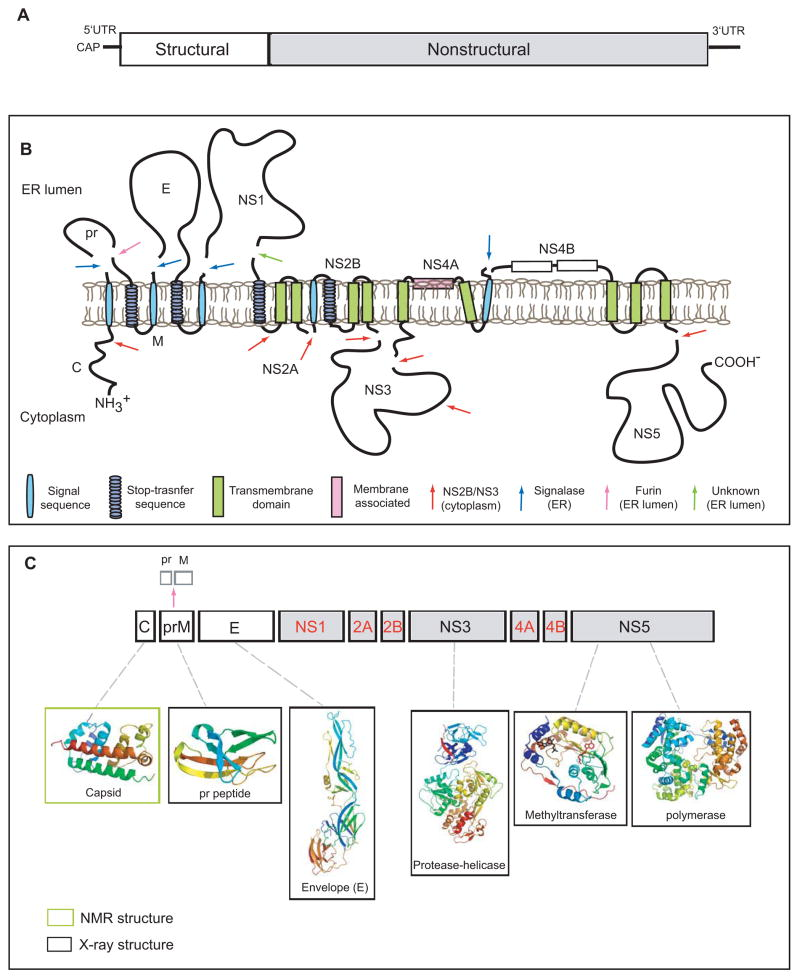
\includegraphics[scale=1]{Images/Dengue_virus_overview.jpg}
  \caption{\citetitle{perera_structural_2008} \cite{perera_structural_2008}}
  \label{fig:Dengue_virus_overview}
\end{figure} \\

Dengue-Viren sind Arboviren, die haupts\"achlich durch Stechm\"ucken, insbesondere die Asiatische Tigerm\"ucke (Aedes albopictus), auf den Menschen \"ubertragen werden \cite{cramer_dengue-virus_2014}. Sie geh\"oren zu einer Gruppe von Erregern, die urspr\"unglich in den Tropen verbreitet waren, aber zunehmend auch in andere Regionen, einschlie\ss{}lich Europa, verschleppt werden \cite{cramer_dengue-virus_2014}. Dengue-Viren haben sich im Zuge der Globalisierung ausgebreitet und gelten als ``Gewinner der Globalisierung'' \cite{meyding-lamade_winners_2018}.
Sie verursachen Dengue-Fieber und in schwereren F\"allen das H\"amorrhagische Dengue-Fieber, das als eine der t\"odlichen Pandemien des 20. Jahrhunderts bezeichnet wird \cite{kuhnle_dengue-fieber_1999}. Auch in Deutschland werden immer mehr Dengue-Fieber-F\"alle aufgezeichnet Abbildung \ref{fig:Dengue_virus_infektionszahlen_deutschland}. Dengue-Viren sind besonders geschickt darin, das menschliche Immunsystem zu \"uberlisten. Sie haben "`perfide Tricks"' entwickelt, um der Immunabwehr zu entgehen \cite{janisch_klein_2017}. In Deutschland wird eine Virus-Surveillance in Stechm\"ucken durchgef\"uhrt, um potenzielle Infektionsherde fr\"uhzeitig zu erkennen \cite{cramer_dengue-virus_2014}. Die zunehmende Verbreitung von Dengue-Viren und ihren Vektoren, insbesondere durch den internationalen Reise- und Warenverkehr, stellt eine wachsende Herausforderung f\"ur das Gesundheitswesen dar, auch in Regionen, die traditionell nicht als Risikogebiete galten \cite{cramer_dengue-virus_2014}. 

\begin{figure}[htpb]
  \centering
  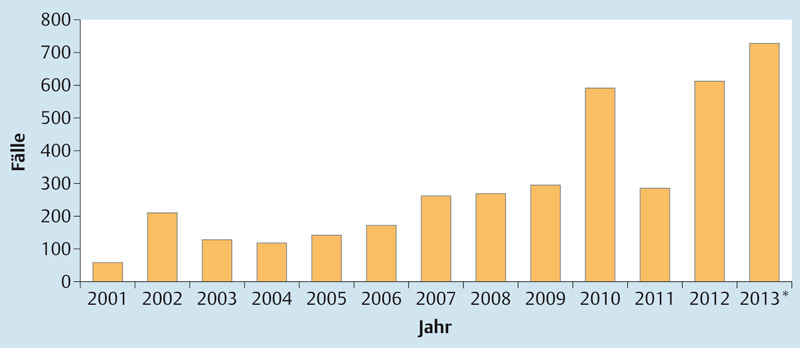
\includegraphics[scale=0.5]{Images/infektionszahlen_dengue_virus_deutschland.jpeg}
  \caption{\citetitle{cramer_dengue-virus_2014} \cite{cramer_dengue-virus_2014}}
  \label{fig:Dengue_virus_infektionszahlen_deutschland}
\end{figure}

Es ist wichtig, die Mutationen der Virenfamilie zu untersuchen und Vorhersagen \"uber die Bereiche zu machen, in denen das Virus eher mutieren kann und wo eher nicht, da Viren, wie die Dengue-Viren, Meister darin sind, das Immunsystem des Menschen zu \"uberlisten. Durch Mutationen k\"onnen sie sich besser an neue Wirte und Umgebungen anpassen, was ihre Verbreitung erleichtert und die Bek\"ampfung erschwert \cite{cramer_dengue-virus_2014}\cite{janisch_klein_2017}. Das Verst\"andnis der Mutationsmuster hilft bei der epidemiologischen \"Uberwachung. Wenn bekannt ist, welche Bereiche des Virusgenoms stabil sind und welche zu Mutationen neigen, k\"onnen Gesundheitsbeh\"orden besser absch\"atzen, wann und wo neue Ausbr\"uche auftreten k\"onnten. Dies ist besonders wichtig in Regionen, in denen invasive Stechm\"uckenarten wie Aedes albopictus nachgewiesen wurden, die als Vektoren f\"ur verschiedene Viren dienen k\"onnen \cite{cramer_dengue-virus_2014}. Die F\"ahigkeit, Mutationen vorherzusagen, kann helfen, potenzielle Pandemien fr\"uhzeitig zu erkennen und Ma\ss{}nahmen zu ergreifen, bevor sich das Virus weit verbreitet \cite{janisch_klein_2017}. Durch die Identifikation stabiler und variabler Regionen des Virusgenoms k\"onnen stabilere Impfstoffe und gezieltere Therapien entwickelt werden. Bei der Entwicklung von Impfstoffen und Medikamenten ist es wichtig absch\"atzen zu k\"onnen, welche Teile des Virus mutieren, da Impfstoffe und antivirale Therapien oft auf spezifische Teile des Virus zielen. Wenn diese Teile mutieren, k\"onnen Impfstoffe und Medikamente weniger wirksam werden \cite{janisch_klein_2017}. 
Insgesamt erm\"oglicht die Untersuchung von Virusmutationen eine proaktive und gezielte Reaktion auf virale Bedrohungen, was entscheidend f\"ur den Schutz der \"offentlichen Gesundheit ist.

\section{Hydropathie und polar requirements}
Hyropathiewerte wurden nachtr\"aglich h\"andisch ver\"andert -> 4 Werte (3 davon leicht, 1 sehr viel)

Hydropathie beschreibt die Affinit\"at eines Molek\"uls zu Wasser. Molek\"ule k\"onnen als hydrophil (wasserliebend) oder hydrophob (wasserabweisend) klassifiziert werden. Diese Eigenschaften beeinflussen, wie Molek\"ule in biologischen Systemen interagieren, insbesondere in Bezug auf Membranproteine und deren Funktion. Jedes Molek\"ul hat ein charakteristisches Hydropathie-Profil, das als eine Art "`Fingerabdruck"' f\"ur seine Struktur betrachtet werden kann. Diese Profile werden h\"aufig verwendet, um die Struktur und Funktion von Membranproteinen zu analysieren und um Beziehungen zwischen verschiedenen Transportproteinen zu identifizieren. In biologischen Systemen spielen hydrophobe und hydrophile Wechselwirkungen eine entscheidende Rolle bei der Faltung von Proteinen, der Bildung von Zellmembranen und der Funktion von Enzymen. Das Verst\"andnis dieser Eigenschaften hilft bei der Vorhersage, wie Molek\"ule in zellul\"aren Umgebungen interagieren. Hydropathie-Analysen werden in der Bioinformatik und Strukturbiologie eingesetzt, um die Topologie von Membranproteinen vorherzusagen und deren funktionelle Eigenschaften besser zu verstehen. Zusammenfassend ist die Hydropathie eine grundlegende chemische Eigenschaft, die entscheidend f\"ur das Verst\"andnis der Molek\"ulinteraktionen in biologischen Systemen ist. Da sie die grundlegenden Molek\"uleigenschaften des Proteins beschreibt. 

Im chemischen Kontext beziehen sich "`polar requirements"' auf die spezifischen Eigenschaften und Bedingungen, die f\"ur polare Molek\"ule oder chemische Verbindungen erforderlich sind, um in einer bestimmten Umgebung stabil zu sein oder zu interagieren. Diese Anforderungen k\"onnen die Polarit\"at, L\"oslichkeit, Wechselwirkungen mit anderen Molek\"ulen und die F\"ahigkeit zur Bildung von Wasserstoffbr\"ucken umfassen. Molek\"ule mit polaren Gruppen (z. B. Hydroxyl- oder Carboxylgruppen) haben unterschiedliche Eigenschaften im Vergleich zu unpolaren Molek\"ulen. Die Polarit\"at beeinflusst, wie Molek\"ule in L\"osungsmitteln interagieren, insbesondere in w\"assrigen L\"osungen. Polare Molek\"ule sind in polaren L\"osungsmitteln wie Wasser besser l\"oslich. Die polar requirements helfen zu bestimmen, welche Molek\"ule in bestimmten chemischen Reaktionen oder biologischen Prozessen effektiv interagieren k\"onnen. Die polar requirements sind entscheidend f\"ur die Vorhersage von Wechselwirkungen zwischen Molek\"ulen, wie z. B. zwischen Enzymen und Substraten oder zwischen Rezeptoren und Liganden. In der Biochemie sind die polar requirements wichtig f\"ur das Verst\"andnis der Struktur und Funktion von Biomolek\"ulen, einschlie\ss{}lich Proteinen und Nukleins\"auren. Auch polar requirements sind entscheidend f\"ur das grundlegende Verst\"andnis der Molek\"uleigenschaften eines Proteins. Obwohl Hydropathie und polar requirements \"ahnliche Eigenschaften untersuchen, zeigt sich bei den Werten einige unterschiede. Da nicht alle Aminos\"auren einduetig zu klassifiezieren sind, wenn man nur eine der beiden Molek\"uleigenschaften verwendet und somit wertvolle Information \"uber die Struktur des Proteins verloren geht, verwenden wir beide Werte f\"ur die Auswertung. 

\section{Biopython}

\section{T-Coffee}
T-Coffee (Tree-based Consistency Objective Function for Alignment Evaluation) is a multiple sequence alignment tool widely used in bioinformatics for aligning DNA, RNA, and protein sequences. T-Coffee works by employing an alignment strategy combined with a consistency-based scoring function. The algorithm for T-Coffee is primarily described in the original publication \citetitle{poirot_tcoffeeigs_2003} \cite{poirot_tcoffeeigs_2003}. The algorithm has the following main steps. T-Coffee first generates all possible pairwise alignments between the input sequences using global and local alignment methods. It then builds a primary library of alignment information from these pairwise alignments, assigning weights to each aligned residue pair based on their consistency across different alignments. The primary library is extended by incorporating transitive alignments, which helps in capturing indirect relationships between sequences. Using the extended library, T-Coffee constructs a guide tree and performs a progressive alignment, aligning the most similar sequences first and gradually adding more distant sequences. The initial alignment is iteratively refined to improve its overall quality and consistency.
T-Coffee is known for its high accuracy, especially when dealing with short sequences. It has been benchmarked against other alignment tools and has shown to produce alignments with accuracy comparable to or better than other methods like MUSCLE \cite{Edgar2004MUSCLEL}.

\chapter{Die Pipeline}
Um die Mutationen zu z\"ahlen nutzen wir aktuell einen sehr naiven Ansatz, indem wir f\"ur alle Sequenzen nur schauen, ob an einer Stelle alle Aminos\"auren gleich sind oder ob es mindestens eine Sequenz gibt, in der es eine andere Aminos\"aure an der Stelle gibt. Wir z\"ahlen nicht, wie viele verschiedene Aminos\"auren es an der Stelle gibt. Wenn wir also eine Mutation z\"ahlen, meine wir, dass an der jeweiligen Stelle mindestens eine Sequenz eine andere Aminos\"aure aufweist, als die Aminos\"aure in der ersten Sequenz. 

Bei der Berechnung der Scores schauen wir immer nach den Extremwerten, also dem minimalen Wert und dem maximalen Wert, die die Aminos\"auren bei den polar requirements, bzw. bei der Hydropathie erreichen. Da auch gaps einen Wert vergeben bekommen (immer den mittleren Wert \"uber alle Werte der beiden Skalen), kann es dazu kommen, dass sich hierdurch an manchen Stellen extremere Werte aufgezeichnet werden, als wenn man nur die tats\"achlich existierenden Aminos\"auren an der jeweiligen Stelle vergleicht. Man muss dabei aber bedenken, dass gaps eine Folge von Mutationen sind und somit auch bei der Berechnung des Scores beachtet werden k\"onnen. Ob dies jedoch sinnvoll ist, bei der Berechnung der Scores und nicht bei der Mutationsz\"ahlung ist fraglich. 

\begin{figure}[htpb]
  \centering
  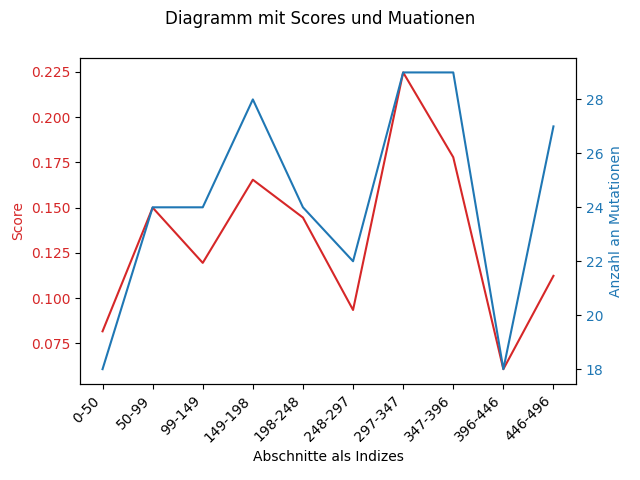
\includegraphics[scale=0.75]{Images/Diagramm_Scores_und_Mutationen_Dengue_viren.png}
  \caption{Diagramm: Scores und Mutationen Dengue viren automatische Auteilung der Sequenzen in 10 gleich gro\ss{}e Bereiche}
  \label{fig:Dengue_virus_scores_and_mutations}
\end{figure}

\chapter{Zusammenfassung und Ausblick}
% In a German thesis write: \subsection{Zusammenfassung und Ausblick}


% !!!!!!!!!!!!!!!!!!!!!!!!!!!!!!!!!!
% !!! Your action is needed here !!!
% !!!!!!!!!!!!!!!!!!!!!!!!!!!!!!!!!!
%
% Replace the following with your conclusion



% Normally, the bibliography comes next at this point. Do *not* (try
% to) include further indices and tables like an index or
% a list of figures or a list of tables or such things. Nobody
% actually uses them and they just use up space. 
%
% You *can* however include a glossary, if this seems appropriate. It
% goes here as an unnumbered chapter. Most thesis will *not* need a
% glossary: a well-written text (re)explains strange words and
% concepts as necessary. However, there are situations where a
% glossary may be helpful.














%%%
% 
% Bibliographies
%
%%%
%
% The uzl-thesis class will load biblatex for the bibliography
% management. This is a powerful package, see its documentation for
% details. The styles will be setup correctly and automatically by
% choosing one of the two style keys as described earlier.
%
% In order for the bibliography to work, run latex in the following
% order (which is the standard order):
% 
% > lualatex thesis-example
% > bibtex thesis-example
% > lualatex thesis-example
% 
% Add BibTeX files using \addbibresource or use the {bibtex entries}
% environment (see below).
%
%%%
%
% Although everyting is normally setup automatically, you can change
% the options passed to biblatex using the key 'biblatex';
% for instance,
%
%   \UzLThesisSetup{biblatex={firstinits=false}}
%
% will switch off shortened first names. Normally, you will not need
% this key in your preamble. 
% 
% Note that the bibtex program is used as the 'backend' of biblatex
% by default (rather than biber, which is the preferred program of
% biblatex). This means that you can (and must) run *bibtex* after you
% have run lualatex on your thesis. If you wish to use biber instead
% of bibtex, say 'biblatex={backend=biber}'. 
% 
%%%
%
% The following environment is optional. It allows you to keep the
% bibtex entries for your thesis right here in the thesis file. What
% happens is that each time this tex file is processed, the contents
% of the following environment gets written to the file
% \jobname-bibtex-entries.bib (this file gets overwritten each
% time). Independently, \addbibresource{\jobname-bibtex-entries.bib}
% is always called if the file \jobname-bibtex-entries.bib
% exists. 
%
% In result, you can edit and keep the bibliography's bibtex entries
% right here. If you change something here, run latex, then bibtex,
% then latex once more.
%
% If you would like to manage the bibtex entries in a separate file,
% remove the below environment, delete the \jobname-bibtex-entries.bib
% file and instead write
%
% \addbibresource{filename-of-your-bibtex-file.bib}
%
% in the preamble.
%
%%%


% !!!!!!!!!!!!!!!!!!!!!!!!!!!!!!!!!!
% !!! Your action is needed here !!!
% !!!!!!!!!!!!!!!!!!!!!!!!!!!!!!!!!!
%
% Replace following example entries with the ones of your thesis.

\begin{bibtex-entries}

@Article{Edgar2004MUSCLEL,
  title={MUSCLE : Low-complexity multiple sequence alignment with T-Coffee accuracy},
  author={Robert C. Edgar and Roque Moraes and Mill Valley},
  year={2004},
  url={https://api.semanticscholar.org/CorpusID:11171007}
}

@Article{poirot_tcoffeeigs_2003,
	title = {Tcoffee@igs: a web server for computing, evaluating and combining multiple sequence alignments},
	volume = {31},
	issn = {0305-1048},
	shorttitle = {Tcoffee@igs},
	url = {https://www.ncbi.nlm.nih.gov/pmc/articles/PMC168929/},
	number = {13},
	urldate = {2024-07-17},
	journal = {Nucleic Acids Research},
	author = {Poirot, Olivier and O'Toole, Eamonn and Notredame, Cedric},
	month = jul,
	year = {2003},
	pmid = {12824354},
	pmcid = {PMC168929},
	pages = {3503--3506}
}

@article{perera_structural_2008,
	title = {Structural {Proteomics} of {Dengue} {Virus}},
	volume = {11},
	issn = {1369-5274},
	url = {https://www.ncbi.nlm.nih.gov/pmc/articles/PMC2581888/},
	doi = {10.1016/j.mib.2008.06.004},
	number = {4},
	urldate = {2024-08-07},
	journal = {Current opinion in microbiology},
	author = {Perera, Rushika and Kuhn, Richard J.},
	month = aug,
	year = {2008},
	pmid = {18644250},
	pmcid = {PMC2581888},
	pages = {369--377},
}

@article{cramer_dengue-virus_2014,
	title = {Dengue-{Virus} \& {Co}.: {Sind} durch {Stechm\"ucken} \"ubertragene {Viren} auf dem {Vormarsch}?},
	volume = {139},
	copyright = {\textcopyright Georg Thieme Verlag KG Stuttgart \cdot New York},
	issn = {0012-0472, 1439-4413},
	shorttitle = {Dengue-{Virus} \& {Co}.},
	url = {http://www.thieme-connect.de/DOI/DOI?10.1055/s-0033-1359968},
	doi = {10.1055/s-0033-1359968},
	abstract = {Thieme E-Books \& E-Journals},
	language = {de},
	number = {06},
	urldate = {2024-08-08},
	journal = {DMW - Deutsche Medizinische Wochenschrift},
	author = {Cramer, J. P. and Schmidt-Chanasit, J.},
	month = feb,
	year = {2014},
	note = {Company: \textcopyright Georg Thieme Verlag KG
Distributor: \textcopyright Georg Thieme Verlag KG
Institution: \textcopyright Georg Thieme Verlag KG
Label: \textcopyright Georg Thieme Verlag KG
Publisher: \textcopyright Georg Thieme Verlag KG},
	pages = {247--250},
}
@article{meyding-lamade_winners_2018,
	title = {[{Winners} of globalization: dengue viruses and {Japanese} encephalitis virus-{Diseases} in neurology]},
	volume = {89},
	issn = {1433-0407},
	shorttitle = {[{Winners} of globalization},
	doi = {10.1007/s00115-018-0616-z},
	language = {ger},
	number = {12},
	journal = {Der Nervenarzt},
	author = {Meyding-Lamad\'e, U. and Craemer, E. M.},
	month = dec,
	year = {2018},
	pmid = {30251003},
	pages = {1338--1343},
}

@inproceedings{janisch_klein_2017,
	title = {Klein und gemein. {Die} perfiden {Tricks} der {Viren}},
	url = {https://heiup.uni-heidelberg.de/journals/index.php/rupertocarola/article/view/23760},
	doi = {10.17885/HEIUP.RUCA.2017.11.23760},
	language = {de},
	urldate = {2024-08-08},
	booktitle = {Ruperto {Carola}},
	publisher = {Ruperto Carola},
	author = {J\"anisch, Thomas and Bartenschlager, Ralf},
	month = dec,
	year = {2017},
	pages = {Nr. 11 (2017): Schein \& Sein},
	annote = {SeriesInformation
Ruperto Carola, Nr. 11 (2017): Schein \& Sein},
}

@article{kuhnle_dengue-fieber_1999,
	title = {Dengue-{Fieber} und {H\"amorrhagisches} {Dengue}-{FieberDie} t\"odliche {Pandemie} des 20.{Jahrhunderts}: {Die} t\"odliche {Pandemie} des 20.{Jahrhunderts}},
	volume = {147},
	copyright = {http://www.springer.com/tdm},
	issn = {0026-9298, 1433-0474},
	shorttitle = {Dengue-{Fieber} und {H\"amorrhagisches} {Dengue}-{FieberDie} t\"odliche {Pandemie} des 20.{Jahrhunderts}},
	url = {http://link.springer.com/10.1007/s001120050397},
	doi = {10.1007/s001120050397},
	language = {de},
	number = {1},
	urldate = {2024-08-08},
	journal = {Monatsschrift Kinderheilkunde},
	author = {Kuhnle, U. and Krahl, W.},
	month = jan,
	year = {1999},
	pages = {48--50},
}


\end{bibtex-entries}



% If you need to have an appendix (I advise against it), insert it
% here using, first, \appendix and then \chapter and then,
% possibly, \section. 
%
% \appendix
%
% \chapter{Technical Appendix}
%
% \section{Experimental Parameters} % possibly
%
% Again, I advise against using an appendix.


\end{document}

%  LocalWords:  LaTeX tex moretexcs Lübeck pdf uzl lualatex bibtex th
%  LocalWords:  TechReport Kernighan Lamport's Tantau's Tantau cls kZ
%  LocalWords:  Mustermann emacs oldschool pdflatex texmf utf biber
%  LocalWords:  biblatex Alphabetische Bibliographie Numerische VIIa
%  LocalWords:  varioref german Einleitung Beiträge dieser Arbeit xml
%  LocalWords:  Ergebnisse Verwandte Arbeiten Aufbau nucleotide VIIc
%  LocalWords:  ensembl amino phylogenetic Alexa Siri decrypt versa
%  LocalWords:  cryptographic pre nondeterministic deterministically
%  LocalWords:  Beutelspacher Untersuchungen zum genetischen sep llcc
%  LocalWords:  Beispiel tikz jpg png Alegrya Kasimir Malewitsch PGF
%  LocalWords:  Lamport Institut für Theoretische Informatik zu url
%  LocalWords:  Universität Springer DowneyF Downey Parameterized doi
%  LocalWords:  BibLaTeX Kime Philipp urldate Mittelbach hyperref Lua
%  LocalWords:  Rahtz Oberdiek Heiko Braams Bezos López fontspec Das
%  LocalWords:  Arseneau amsmath ist Tipps und zur Formulierung
%  LocalWords:  mathematischer Gedanken Mathematik Studienanfänger
%  LocalWords:  Albrecht Vieweg Teubner Verlag
